\UseRawInputEncoding
% Tipo de documento y paquetes a utilizar.
\documentclass[12pt]{article}
\usepackage[utf8]{inputenc}
\usepackage{amsmath, amsthm, amsfonts, mathtools}	% Paquete para usar más fórmulas y ecuaciones.
\usepackage{graphicx}								% Paquete para usar imágenes y figuras.
\usepackage{array}									% Paquete para fijar un ancho de columna.
\usepackage{multirow}								% Paquete para combinar filas de tablas.
\usepackage{geometry} 								% Paquete para trabajar con los márgenes del documento.
\usepackage{fancyhdr}								% Paquete para personalizar encabezado y pie de página.
\usepackage{lastpage}								% Paquete para reverenciar páginas del documento.
\usepackage{tabularx}								% Paquete para fijar un ancho de tabla.
\usepackage{listings} 								% Paquete para escribir código de programación.
\usepackage{inconsolata}							% Paquete de tipo de letra consola.
\usepackage{xcolor}                                 % Paquete básico para agregar color al texto.
\usepackage{float}          						% paquete para utilizar fijación de figuras H.
\usepackage{comment}                                % Paquete para comentar varias líneas a la vez.
\usepackage{hyperref}                               % Paquete para insertar links en el documento.
\usepackage[style=apa]{biblatex}					% Paquete para usar referencias y citas.
\addbibresource{referencias.bib}					% Se agrega el archivo .bib al documento.

% Define colores nuevos.
\definecolor{color}{HTML}{E4E4EE}
\definecolor{verde}{HTML}{3C8031}

% Personalización de la fuente para el código.
\lstset{
    language = TeX,                     % Lenguaje con palabras reservadas de este resaltadas.
    basicstyle = \ttfamily\footnotesize,% Utiliza la fuente tttfamily, en especial el paquete inconsolata.
    frame = single,                     % Quita el marco al cuadro flotante que contiene el código o texto.
    backgroundcolor = \color{color},    % Cambia el color del fondo del marco del código. Utiliza el paquete "xcolor" y define un nuevo color.
    columns = fullflexible,             % Ajusta el cuadro flotante al tamaño del texto del documento.
    breaklines = true,                  % Ajusta el texto dentro del contenedor.
    inputencoding = utf8,               % Admite caracteres del código UTF8.
    extendedchars = true,               % Soporte para caracteres especiales.
    %numbers = left,                    % Agrega número de línea al código (izquierda, sin número y derecha).
    showstringspaces = false,           % Quita los guiones bajos predeterminados de los espacios en cadenas de texto.
    escapebegin = \obeyspaces,          % Complemento de la entrada anterior.
    % rulecolor = \color{red},          % Color del borde del marco del código.
    % numberstyle = \color{red},        % Color de los números en el texto o código.
    % stringstyle = \color{red},        % Color de las cadenas de texto en el texto o código.
    % keywordstyle = \color{red},       % Color de las palabras reservadas en el texto o código.
    % identifierstyle = \color{red},    % Color del texto o código.
    commentstyle = \color{verde},       % Color de los comentarios en el texto o código.
    literate =                          % Acepta los siguientes caracteres especiales fuera de UTF8.
        {á}{{\'a}}1 {é}{{\'e}}1 {í}{{\'i}}1 {ó}{{\'o}}1 {ú}{{\'u}}1
        {Á}{{\'A}}1 {É}{{\'E}}1 {Í}{{\'I}}1 {Ó}{{\'O}}1 {Ú}{{\'U}}1
        {ñ}{{\~n}}1 {Ñ}{{\~N}}1,
}

% Márgenes del documento.
\newgeometry{
    top=2.5cm,     % Superior.
    bottom=2.5cm,  % Inferior.
    outer=2.5cm,   % Parte exterior.
    inner=2.5cm,   % Parte interior.
}

% Personalización de la cabecera y pie de página.
\pagestyle{fancy}
\fancyhf{}
\rhead{Overleaf}                                            % Texto en esquina superior derecha.
\lhead{Apuntes de LaTeX}                                    % Texto en esquina superior izquierda.
\rfoot{Pagina \thepage \hspace{1pt} de \pageref{LastPage}}  % Texto en esquina inferior derecha (Página n de n).
% Ancho de línea horizontal superior e inferior.
\renewcommand{\headrulewidth}{1pt}
\renewcommand{\footrulewidth}{1pt}

% Datos de la portada.
\title{Apuntes de LaTeX}
\author{migueluisV}
\date{Actualizadas: Mayo 2023}

% Inicio del documento.
\begin{document}

% cambia los títulos de los índices:
% Content - Índice
% List of Tables - Índice de Tablas
% List of Figures - Índice de Figuras
\renewcommand*\contentsname{Índice}
\renewcommand{\listtablename}{Índice de Tablas}
\renewcommand{\listfigurename}{Índice de Figuras}

% Agrega portada e índices.
\maketitle\newpage
\tableofcontents\newpage
\listoffigures\newpage
\listoftables\newpage

% Archivos que conforman al documento.
Todas la información y comandos usados para crear y ejemplificar este documento fueron sacados de los enlaces puestos en la sección de referencias: (\textit{\cite{trefor2}}), (\textit{\cite{trefor1}}), (\textit{\cite{overl}}).



\section{Comandos básicos y estructura del documento}

Para trabajar con \LaTeX es necesario tener conocimiento de sus nociones básicas y cómo estructurarlo para un mejor orden.


\subsection{Lo básico}
\begin{itemize}
    \item \textbf{Inicio de comando}: para iniciar un comando en \LaTeX  se utiliza una diagonal (\textbf{\textbackslash}). Por ejemplo:
    \begin{center}
        \textit{\textbackslash{textbackslash}, \textbackslash{par}, \textbackslash{LaTeX}}
    \end{center}
    \item \textbf{Salto de línea}: para hacer un salto de línea, se usan las dos \textbf{\textbackslash\textbackslash} o dándo doble ENTER con el teclado (dos salto de líneas).
    \item \textbf{Salto de página}: para hacer un salto de página se usa el comando \textbf{\textbackslash{newpage}}.
    \item \textbf{Sangría}: Al dejar una línea vacía antes de un párrafo, este tendrá sangría por defecto en \LaTeX. De igual manera, con el comando \textbf{\textbackslash{hspace\{\}}} podemos insertar una sangría a un párrafo, esta sangría debe ser establecida con alguna de las unidades que maneja \LaTeX, que veremos a continuación.
    \item Un párrafo puede ser creado simplemente escribiendo en el archivo \textit{.tex} después del comienzo del documento, sin embargo, un comando para crear párrafos de una forma más ordenada y con un ancho de párrafo es \textbf{\textbackslash{parbox\{\}\{\}}}, donde el primer par de llaves contiene el ancho del párrafo, y el segundo par contiene el texto de párrafo:
    \begin{lstlisting}
        \begin{document}
            Esto es un párrafo normal y corriente.

            \parbox{10cm}{Esto es un párrafo con 10cm de ancho}
        \end{document}
    \end{lstlisting}
\end{itemize}


\subsection{Unidades y longitud}

Para poder establecer el alto o ancho de una imagen, columna, celda, figura, debemos establecer dicha medida de ancho o alto, para ello, requerimos de unidades que \LaTeX conoce y así, establecer el tamaño que deseamos, a continuación está la lista de unidades que se manejan:
\begin{itemize}
    \item \textbf{pt}: puntos, que son aproximadamente 0.3515 milímetros.
    \item \textbf{mm}: milímetros.
    \item \textbf{cm}: centímetros.
    \item \textbf{in}: pulgadas, que son 2.54 centímetros.
    \item \textbf{ex}: el alto de una "x" minúscula dependiendo de la fuente con la que se esté trabajando.
    \item \textbf{em}: el ancho de una "m" mayúscula dependiendo de la fuente con la que se esté trabajando.
    \item \textbf{mu}: su valor es igual a $\frac{1}{18}$em.
    \item \textbf{sp}: punto especial, 65,536 puntos especiales son iguales a 1pt.
\end{itemize}

De igual forma, existen algunos comandos de longitud especiales para no rompernos la cabeza utilizando las unidades, los cuales son:
\begin{itemize}
    \item \textbf{\textbackslash{columnwidth}}: el ancho de una columna.
    \item \textbf{\textbackslash{paperwidth}}: el ancho de toda la página.
    \item \textbf{\textbackslash{paperheight}}: el alto de toda la página.
    \item \textbf{\textbackslash{parskip}}: el espacio vertical entre párrafos.
    \item \textbf{\textbackslash{textwidth}}: el ancho del texto del documento.
    \item \textbf{\textbackslash{textheight}}: el alto del texto del documento
    \item \textbf{\textbackslash{topmargin}}: el largo del margen superior.
\end{itemize}

Un ejemplo de la aplicación de los comandos de longitud o unidades de longitud de \LaTeX se encuentra a continuación:
\begin{lstlisting}
    \usepackage{graphicx}
    
    \begin{document}
        \includegraphics[width=\textwidth]{abc.png}
        \includegraphics[height=5cm]{cba.png}
    \end{document}
\end{lstlisting}

\textit{Nota}: sea cuidadoso con asignar tamaños a objetos de \LaTeX, puede asignarle el tamaño del margen a un objeto y que sobresalga de la página.


\subsection{Títulos, subtítulos y tablas de contenido}

\textbf{Títulos y subtítulos}

Los títulos y subtítulos en \LaTeX  dan un orden y estructura al documento que se está trabajando:
\begin{itemize}
    \item \textbf{\textbackslash{section}\{\}}: crea un título o sección.
    \item \textbf{\textbackslash{subsection\{\}}}: crea un subtítulo o subsección.
    \item \textbf{\textbackslash{subsubsection\{\}}}: crea un subtítulo del subtítulo.
\end{itemize}
\begin{lstlisting}
    \begin{document}
        \section{Título 1}
        \subsection{Título 1.1}
        \subsection{Título 1.1.1}
    \end{document}
    
    
    Despliega:
    1 Título 1
    1.1 Título 1.1
    1.1.1 Título 1.1.1
\end{lstlisting}

\textbf{Tablas de contenido}

Para que se cree correctamente una índice de contenido, ya sea de todo el documento, imágenes, figuras o tablas, es necesario establecer en los puntos donde, se requiere de las secciones, subsecciones y etiquetas de objetos para crear títulos, subtítulos y así sucesivamente, de los índices; por lo general, estos índices suelen colocarse enseguida del inicio del documento. Se utilizan los siguientes comandos:
\begin{itemize}
    \item Índice:
    \begin{itemize}
        \item \textbf{\textbackslash{tableofcontents}}: crea un índice del documento.
        \item \textbf{\textbackslash{renewcommand*} y \textbackslash{contentsname}}: juntos, cambian el título del índice del documento (que originalmente es "Contents").
        \begin{lstlisting}
            \begin{document}
                \renewcommand*\contentsname{Índice}
                \tableofcontents
            \end{document}
        \end{lstlisting}
    \end{itemize}
    \item Índice de tablas:
    \begin{itemize}
        \item \textbf{\textbackslash{listoftables}}: crea un índice de tablas.
        \item \textbf{\textbackslash{renewcommand\{\}\{\}}}: cambia el título del índice de tablas.
        \begin{lstlisting}
            \begin{document}
                \renewcommand{listtablename}{Índice de Tablas}
                \listoftables
            \end{document}
        \end{lstlisting}
    \end{itemize}
    \item Índice de figuras:
    \begin{itemize}
        \item \textbf{\textbackslash{listoffigures}}: crea un índice de figuras.
        \item \textbf{\textbackslash{renewcommand\{\}\{\}}}: cambia el título del índice de figuras.
        \begin{lstlisting}
            \begin{document}
                \renewcommand{listfigurename}{Índice de Figuras}
                \listoffigures
            \end{document}
        \end{lstlisting}
    \end{itemize}
    \item Índice de ecuaciones: esta opción no está disponible de forma nativa.
\end{itemize}


\subsection{Márgenes}

Debemos agregar el paquete \textbf{geometry} dentro de nuestro documento para poder modificar los márgenes del mismo.

Entonces, previo a darle comienzo al documento, usamos el comando \textbf{newgeometry} y, dentro de sus llaves, agregamos los valores que queremos que tengan nuestros márgenes; los parámetros que puede recibir son: \textbf{top}, \textbf{bottom}, \textbf{outer} e \textbf{inner} (\textit{arriba}, \textit{abajo}, \textit{la parte exterior del documento} y \textit{la parte interior}; si estuviéramos viendo el documento como un libro, la parte outer de la página izquierda sería la izquierda, y la parte inner sería el lad derecho, para la página derecha, el outer es el lado derecho y el inner la izquierda de la página; para un documento digital, que se desliza hacía abajo, el outer es el lado derecho y el inner el izquierdo), el valor que se le asigne a estos parámetros tiene que ser un unidades utilizadas por \LaTeX.
\begin{lstlisting}
    \usepackage{geometry} % Paquete para trabajar con los márgenes del documento.
    
    % Márgenes del documento.
    \newgeometry{
        top=2.5cm,     % Superior.
        bottom=2.5cm,  % Inferior.
        outer=2.5cm,   % Parte exterior.
        inner=2.5cm,   % Parte interior.
    }
    
    \begin{document}
    
    \end{document}
\end{lstlisting}

El resultado del ejemplo anterior se puede ver a lo largo de los márgenes de este documento.


\subsection{Encabezado y pie de página}

\LaTeX por defecto maneja el encabezado y pie de página solamente con el número de página, esto es porque el documento utiliza el comando \textbf{\textbackslash{pagestyle\{\}}} que define que es lo qué contendrá ambas partes del documento, suele estar ubicado antes del inicio del documento, su estilo por defecto es \textit{plain}, pero se le puede poner otro tipo estilo, como:
\begin{itemize}
    \item \textbf{plain}: estilo predeterminado de \LaTeX, simplemente agrega el número de página al documento.
    \item \textbf{myheading}: utilizado para documentos con dos lados de página, escribe en la cabecera el título del capítulo en el que se esté posicionado.
    \item \textbf{empty}: deja ambas partes del documento vacío.
    \item \textbf{thispagestyle}: este comando se utiliza para para asignarle un estilo de página a una sola página, esto para diferenciarla de las otras.
\end{itemize}
\begin{center}
    \textit{\textbackslash{pagestyle\{plain\}}}
\end{center}


\subsubsection{Personalización}

Para salirnos de lo básico mostrado en la sección anterior, podemos personalizar aún más el encabezado y pie de página, para ello requerimos el paquete \textbf{fancyhdr}, después, dentro del comando \textbackslash{pagestyle}, le pasamos como parámetro el valor\textbf{fancy}, posterior a ello utilizaremos el comando.

\textbf{\textbackslash{fancyhf\{\}}}, este último funciona para limpiar todo lo que esté contenido en la cabecera y pie (algo así como empty de pagestyle). La siguiente configuración va previa al comienzo del documento:
\begin{lstlisting}
    \usepackage{fancyhdr}	% Paquete para personalizar encabezado y pie de página.
    
    % Personalización de la cabecera y pie de página.
    \pagestyle{fancy}
    \fancyhf{}

    \begin{document}
    
    \end{document}
\end{lstlisting}

Algunos de los parámetros son utilizados en este documento, que se le pueden pasar a \textbf{fancyhdr} son:
\begin{itemize}
    \item \textbf{rhead}: texto del lado derecho del encabezado.
    \item \textbf{chead}: texto en el centro del encabezado.
    \item \textbf{lhead}: texto en el lado izquierdo del encabezado.
    \item \textbf{rfoot}: texto en el lado derecho del pie de página.
    \item \textbf{cfoot}: texto en el centro del pie de página.
    \item \textbf{lfoot}: texto en el lado izquierdo del pie de página.
    \begin{lstlisting}
        \usepackage{fancyhdr}	% Paquete para personalizar encabezado y pie de página.
    
        % Personalización de la cabecera y pie de página.
        \pagestyle{fancy}
        \fancyhf{}
        % Texto en esquina superior derecha.
        \rhead{Overleaf}
        % Texto en esquina superior izquierda.
        \lhead{Apuntes de LaTeX}
        % Texto en la esquina inferior izquierda.
        lfoot{Hola mundo}
        % Texto en esquina inferior derecha (Página n).
        \rfoot{Pagina \thepage}

        \begin{document}
    
        \end{document}
    \end{lstlisting}
    \item \textbf{headrulewidth}: establece una línea vertical en la cabecera, este comando debe usarse como parámetro para el comando \textbf{\textbackslash{renewcommand}}. El grosor de esta línea es el parámetro de este comando y puede establecerse con unidades de medida.
    \item \textbf{footrulewidth}: establece una línea vertical en el pie de página, este comando debe usarse como parámetro para el comando \textbf{\textbackslash{renewcommand}}. El grosor de esta línea es el parámetro de este comando y puede establecerse con unidades de medida.
    \begin{lstlisting}
        \usepackage{fancyhdr}	% Paquete para personalizar encabezado y pie de página.
    
        % Personalización de la cabecera y pie de página.
        \pagestyle{fancy}
        \fancyhf{}
        % Texto en esquina superior derecha.
        \rhead{Overleaf}
        % Texto en esquina superior izquierda.
        \lhead{Apuntes de LaTeX}
        % Texto en la esquina inferior izquierda.
        lfoot{Hola mundo}
        % Texto en esquina inferior derecha (Página n).
        \rfoot{Pagina \thepage}
        % Ancho de línea horizontal superior e inferior.
        \renewcommand{\headrulewidth}{1pt}
        \renewcommand{\footrulewidth}{1pt}

        \begin{document}
    
        \end{document}
    \end{lstlisting}
    \item \textbf{Página x de y}: se puede personalizar el estilo en el que se presenta la numeración de páginas, para ello podemos escribir el texto "Página x de z" donde remplazamos x por el comando \textbf{thepage} y z por \textbf{pageref} donde su parámetro es \textbf{LastPage} (requiere el paquete \textbf{lastpage} para el funcionamiento correcto de esta personalización), con esto obtenemos como resultado que cada página tenga la numeración con el estilo "Página 1 de 120", el estilo de esta presentación puede ser personalizado, lo que importa son los comandos utilizados en este punto, depende de uno escoger si poner este comando en el encabezado o pie.
    \begin{lstlisting}
        \usepackage{fancyhdr}	% Paquete para personalizar encabezado y pie de página.
        \usepackage{lastpage}	% Paquete para reverenciar páginas del documento.
    
        % Personalización de la cabecera y pie de página.
        \pagestyle{fancy}
        \fancyhf{}
        % Texto en esquina superior derecha.
        \rhead{Overleaf}
        % Texto en esquina superior izquierda.
        \lhead{Apuntes de LaTeX}
        % Texto en la esquina inferior izquierda.
        lfoot{Hola mundo}
        % Texto en esquina inferior derecha (Página n de n).
        \rfoot{Pagina \thepage \hspace{1pt} de \pageref{LastPage}}
        % Ancho de línea horizontal superior e inferior.
        \renewcommand{\headrulewidth}{1pt}
        \renewcommand{\footrulewidth}{1pt}

        \begin{document}
    
        \end{document}
    \end{lstlisting}
\end{itemize}

\textit{Nota}: los comandos \textbf{\textbackslash{thepage}} referencia a la página actual en el contador del documento.

El desarrollo de los ejemplos anteriores se ven a lo largo de todos las cabeceras y pies de página de este documento.



\section{Manipulando el texto del documento}

La necesidad de agrandar o encoger la fuente en un documento es algo básico, en \LaTeX se puede saciar esta necesidad. Los tamaños de letra por defecto de este lenguaje son los de 10pt, 11pt y 12pt para tipos de documentos \textit{article} o \textit{report}, siendo 10pt con el que se crea todo nuevo documento, si intentamos poner algún otro valor con otra unidad, se pondrá automáticamente 10pt, por lo que se tendrá que recurrir a paquetes externos.


\subsection{Estilo del texto}

Para resaltar textos se usan los siguientes comandos:
\begin{itemize}
    \item \textbf{Negrita}: se usa el comando \textbf{\textbackslash{textbf\{\}}} para hacer el texto negrita.
    \item \underline{Subrayado}: se usa el comando \textbf{\textbackslash{underline\{\}}} para hacer una subrayar el texto.
    \item \textit{Cursiva}: se usa el comando \textbf{\textbackslash{textit\{\}}} para hacer el texto cursiva.
\end{itemize}
\begin{lstlisting}
    \begin{document}
        \textbf{Este texto es negrita.}
        \textit{Este texto es cursiva.}
        \underline{Este texto está subrayado.}
    \end{document}
\end{lstlisting}


\subsection{Tamaño del texto}


\subsubsection{En todo el documento}

Previo a mostrar la solución de aumentar o reducir la fuente de un documento con un paquete externo, queremos presentar que hay dos formas de cambiar el tamaño del texto del documento \LaTeX, la primera es hacer que todo el texto de todo el documento cambie de tamaño desde la instrucción \textit{documentclass\{\}}, como se ve a continuación:
\begin{lstlisting}
    % Tipo de documento con tamaño de fuente de 12pt.
    % \documentclass[12pt]{article}
\end{lstlisting}

\textit{Nota}: el segundo comando del ejemplo anterior fue comentado porque, a pesar de estar en un bloque de código, el comando se sigue ejecutando a pesar de que no debería ejecutarse.

Como podemos apreciar, utilizamos uno de los tamaños de letra predeterminado de \LaTeX entre corchetes previo al tipo de documento, sin embargo, seguimos limitado a los tamaños 10, 11 y 12 puntos.


\subsubsection{En algunos bloques de texto}

La segunda solución para cambiar el tamaño de la fuente del documento es utilizar las siguientes palabras reservadas o comandos de \LaTeX:
\begin{itemize}
    \item \textbf{\textbackslash{tiny}}: tamaño de letra más pequeño.
    \item \textbf{\textbackslash{scriptsize}}: tamaño un poco mayor a \textit{tiny}.
    \item \textbf{\textbackslash{footnotesize}}: tamaño de letra similar a los textos en pies de página.
    \item \textbf{\textbackslash{small}}: tamaño de letra un poco menor al tamaño de letra predeterminado del documento (10pt, 11pt o 12pt).
    \item \textbf{\textbackslash{normalsize}}: el mismo tamaño que el tamaño de letra predeterminado del documento (10pt, 11pt o 12pt).
    \item \textbf{\textbackslash{large}}: tamaño de letra un poco mayor a \textit{normalsize}.
    \item \textbf{\textbackslash{Large}}: tamaño de letra un poco mayor a \textit{large}.
    \item \textbf{\textbackslash{LARGE}}: tamaño de letra un poco mayor a \textit{Large}.
    \item \textbf{\textbackslash{huge}}: tamaño de letra un poco mayor a \textit{LARGE}.
    \item \textbf{\textbackslash{Huge}}: tamaño de letra un poco mayor a \textit{huge} y el tamaño más grande.
\end{itemize}

Una demostración de estos tamaños en un párrafo es la siguiente:
\begin{lstlisting}
    \tiny lorem ipsum.
    \scriptsize lorem ipsum.
    \footnotesize lorem ipsum.
    \small lorem ipsum.
    \normalsize lorem ipsum.
    \large lorem ipsum.
    \Large lorem ipsum.
    \LARGE lorem ipsum.
    \huge lorem ipsum.
    \Huge lorem ipsum.
\end{lstlisting}
\parbox{\textwidth}{\tiny lorem ipsum.}
\parbox{\textwidth}{\scriptsize lorem ipsum.}
\parbox{\textwidth}{\footnotesize lorem ipsum.}
\parbox{\textwidth}{\small lorem ipsum.}
\parbox{\textwidth}{\normalsize lorem ipsum.}
\parbox{\textwidth}{\large lorem ipsum.}
\parbox{\textwidth}{\Large lorem ipsum.}
\parbox{\textwidth}{\LARGE lorem ipsum.}
\parbox{\textwidth}{\huge lorem ipsum.}
\parbox{\textwidth}{\Huge lorem ipsum.}

Si busca aplicar alguno de estos tamaños a solo unas cuantas palabras de un párrafo, siga el siguiente ejemplo:
\begin{lstlisting}
    {\Large lorem ipsum lorem ipsum lorem ipsum lorem ipsum lorem ipsum} lorem ipsum lorem ipsum lorem ipsum lorem ipsum lorem ipsum lorem ipsum lorem ipsum lorem ipsum lorem ipsum lorem ipsum lorem ipsum lorem ipsum lorem ipsum lorem ipsum lorem ipsum lorem ipsum lorem ipsum lorem ipsum lorem ipsum 
\end{lstlisting}

\textit{{\Large lorem ipsum lorem ipsum lorem ipsum lorem ipsum lorem ipsum} lorem ipsum lorem ipsum lorem ipsum lorem ipsum lorem ipsum lorem ipsum lorem ipsum lorem ipsum lorem ipsum lorem ipsum lorem ipsum lorem ipsum lorem ipsum lorem ipsum lorem ipsum lorem ipsum lorem ipsum lorem ipsum lorem ipsum}

Sea consiente de que estas instrucciones no le permiten ingresar un tamaño y unidad de medida de su preferencia, si desea realizar dicha acción, debe acudir a paquetes externos, como lo muestra este \href{https://www.youtube.com/watch?v=VRp4B1JzHTM}{\textcolor{cyan}{video}}.


\subsection{Color del texto}

Por defecto, \LaTeX no permite utilizar colores para pintar un texto en específico, por lo que tendrá que recurrir a paquetes externos, como lo pueden ser \textbf{color} y \textbf{xcolor}:
\begin{center}
    \textit{
        \textbackslash{usepackage\{color\}} \\
        \textbackslash{usepackage\{xcolor\}}
    }
\end{center}

La principal diferencia entre ambos es que el primer no tiene tantos colores predeterminados por defecto, del mismo modo que no se pueden crear o personalizar colores con tantos modelos (hexadecimal, RGB, RGBA, por ejemplo), mientras que el segundo si tiene estas posibilidad, por lo que recomendamos utilizar el segundo paquete.


\subsubsection{Utilizando colores predeterminados}

Basta con importar el paquete de su preferencia, para fines de este documento y sección se utilizará \textit{xcolor}, y utilizar el comando \textbf{textcolor} para pintar una o varias palabras de otro color:
\begin{lstlisting}
    Este \textcolor{red}{mensaje} tiene \textcolor{blue}{varias} palabras \textcolor{green}{en} distintos \textcolor{purple}{colores}.

    \textcolor{red}{Este mensaje está pintado todo de un color}.
\end{lstlisting}

Este \textcolor{red}{mensaje} tiene \textcolor{blue}{varias} palabras \textcolor{green}{en} distintos \textcolor{purple}{colores}.

\textcolor{red}{Este mensaje está pintado todo de un color}.


\subsubsection{Utilizando colores personalizados}

Si requiere de un color distinto a los disponibles en los paquetes externos, utilice el comando \textbf{definecolor} con los siguientes valores:
\begin{center}
    \textit{\textbackslash{definecolor\{nombre\}\{modelo\}\{configuración\}}}
\end{center}

Donde:
\begin{itemize}
    \item nombre: es el nombre del color que se está creando.
    \item modelo: es la forma en la que se creará el color, pudiendo ser escala de grises (\textit{gray}), \textit{rgb}, \textit{RGB}, \textit{HTML} o cían, magenta, amarillo y negro (\textit{cmyc})
    \item configuración: es la definición o configuración del color. Según el modelo será la configuración, por ejemplo, el modelo HTML utiliza valores hexadecimales como configuración o RGB utiliza un trío de valores para el rojo, verde y azul (0,0,0 por ejemplo).
\end{itemize}

Este documento tiene definido los siguientes colores:
\begin{lstlisting}
    % Define colores nuevos.
    \definecolor{color}{HTML}{E4E4EE}
    \definecolor{verde}{HTML}{3C8031}
\end{lstlisting}

\textcolor{color}{Texto con el color llamado 'color'}.

\textcolor{verde}{Texto con el color llamado 'verde'}.

Ambos colores son utilizados más que nada en las secciones de código de este documento. Puede consultar este \href{https://www.overleaf.com/learn/latex/Using_colours_in_LaTeX#Creating_your_own_colours}{\textcolor{cyan}{enlace}} o \href{https://en.wikibooks.org/wiki/LaTeX/Colors}{\textcolor{cyan}{este otro}} para consultar más información acerca de la creación de colores con xcolor y sus colores predeterminados disponibles.


\subsubsection{Color del fondo del texto}

Siguiendo con la línea de colorear objetos en documentos \LaTeX, también se puede pintar el fondo de un párrafo o texto utilizando el comando \textbf{colorbox}, en conjunto con el uso de colores que se ha explicado previamente.
\begin{lstlisting}
    Esta \colorbox{orange}{palabra} tiene un color de fondo naranja.
\end{lstlisting}

Esta \colorbox{orange}{palabra} tiene un color de fondo naranja.


\subsection{Alineación del texto}

Por defecto, \LaTeX utiliza la alineación de texto \textbf{justificada}, si es necesario alinear nuestro texto a la izquierda, centrado o derecha, se tienen las siguientes opciones.

\textbf{A la izquierda}

Utilice los comandos \textbf{begin\{flushleft\}} y \textbf{end\{flushleft\}} para alinear un texto a la izquierda:
\begin{lstlisting}
    \begin{flushleft}
        lorem ipsum lorem ipsum lorem ipsum lorem ipsum lorem ipsum} lorem ipsum lorem ipsum lorem ipsum lorem ipsum lorem ipsum lorem ipsum lorem ipsum lorem ipsum lorem ipsum lorem ipsum lorem ipsum lorem ipsum lorem ipsum lorem ipsum lorem ipsum lorem ipsum lorem ipsum lorem ipsum lorem ipsum
    \end{flushleft}
\end{lstlisting}
\begin{flushleft}
    lorem ipsum lorem ipsum lorem ipsum lorem ipsum lorem ipsum lorem ipsum lorem ipsum lorem ipsum lorem ipsum lorem ipsum lorem ipsum lorem ipsum lorem ipsum lorem ipsum lorem ipsum lorem ipsum lorem ipsum lorem ipsum lorem ipsum lorem ipsum lorem ipsum lorem ipsum lorem ipsum lorem ipsum 
\end{flushleft}

\textbf{Centrado}

Visto anteriormente para alinear tablas, figuras o mensajes importantes, el comando \textbf{begin\{center\}} y \textbf{end\{center\}} alineará su texto al centro:
\begin{lstlisting}
    \begin{center}
        lorem ipsum lorem ipsum lorem ipsum lorem ipsum lorem ipsum} lorem ipsum lorem ipsum lorem ipsum lorem ipsum lorem ipsum lorem ipsum lorem ipsum lorem ipsum lorem ipsum lorem ipsum lorem ipsum lorem ipsum lorem ipsum lorem ipsum lorem ipsum lorem ipsum lorem ipsum lorem ipsum lorem ipsum
    \end{center}
\end{lstlisting}
\begin{center}
    lorem ipsum lorem ipsum lorem ipsum lorem ipsum lorem ipsum lorem ipsum lorem ipsum lorem ipsum lorem ipsum lorem ipsum lorem ipsum lorem ipsum lorem ipsum lorem ipsum lorem ipsum lorem ipsum lorem ipsum lorem ipsum lorem ipsum lorem ipsum lorem ipsum lorem ipsum lorem ipsum lorem ipsum 
\end{center}

La diferencia entre el comando anterior y \textbf{centering} es que el primero tiene un inicio y fin, mientras que el segundo terminará su efecto hasta que aparezca otro comando que lo interrumpta, es esta razón por la cual se recomienda utilizar \textit{centering} en figuras o tablas, mientras que \textit{center} es recomendado para textos.
\\
\textbf{A la derecha}

Utilice los comandos \textbf{begin\{flushright\}} y \textbf{end\{flushright\}} para alinear un texto a la izquierda:
\begin{lstlisting}
    \begin{flushright}
        lorem ipsum lorem ipsum lorem ipsum lorem ipsum lorem ipsum} lorem ipsum lorem ipsum lorem ipsum lorem ipsum lorem ipsum lorem ipsum lorem ipsum lorem ipsum lorem ipsum lorem ipsum lorem ipsum lorem ipsum lorem ipsum lorem ipsum lorem ipsum lorem ipsum lorem ipsum lorem ipsum lorem ipsum
    \end{flushright}
\end{lstlisting}
\begin{flushright}
    lorem ipsum lorem ipsum lorem ipsum lorem ipsum lorem ipsum lorem ipsum lorem ipsum lorem ipsum lorem ipsum lorem ipsum lorem ipsum lorem ipsum lorem ipsum lorem ipsum lorem ipsum lorem ipsum lorem ipsum lorem ipsum lorem ipsum lorem ipsum lorem ipsum lorem ipsum lorem ipsum lorem ipsum 
\end{flushright}

Consulte \href{https://www.overleaf.com/learn/latex/Paragraphs_and_new_lines#Paragraph_alignment}{\textcolor{cyan}{este enlace}} para tener más información sobre la alineación de texto u las alternativas.


\subsection{Interlineado del texto}

El interlineado en \LaTeX no es algo que le interese a los usuarios, ya que este lenguaje se encarga de ajustar el interlineado al tipo de documento que se esté trabajando, sin embargo, siempre existirá la duda de cómo ajustarlo a nuestra preferencia. Para lograr este cometido, es necesario reescribir el comando que se encarga de ajustar el interlineado de todo el documento. El interlineado actual de este documento es sencillo, por lo que puede tomar estos ejemplos y aplicarlos a su documento.


\subsubsection{En todo el documento}

El comando \textbf{baselinestrech} es el que se encarga de establecer el interlineado de un documento, por defecto, el valor de este comando es 1, veamos como se utiliza.
\begin{lstlisting}
    % Sobre escribe el comando baselinestrech con el valor 2.
    \renewcommand{\baselinestrech}{2}

    % \begin{document}
    % Inicio del documento...
    % \end{document}
\end{lstlisting}

Se utiliza el comando \textit{renewcommand} para sobre escribir un comando anterior, en este caso, \textit{baselinestrech}, el valor que se le puede poner puede ser 1, 1.5, 2, o alguno otro conocido o utilizado en otros editores de texto. Puede consultar este \href{http://elclubdelautodidacta.es/wp/2012/06/latex-modificando-el-espacio-de-interlineado/}{\textcolor{cyan}{enlace}} para más información referente al interlineado.


\subsubsection{En algunos bloques de texto}

Agregamos el paquete \textbf{setspace}, el cual posee los comandos para establecer un interlineado simple (1), de 1.5 y doble (2), con la posibilidad de crear un interlineado propio, de 1.8 por ejemplo.
\begin{center}
    \textit{\textbackslash{usepackage\{setspace\}}}
\end{center}
\begin{lstlisting}
    \doublespacing
    Todo este texto tendrá interlineado doble
    \onehalfspace
    Todo este texto tendrá interlineado uno y medio
    \singlespace
    Todo este texto tendrá interlineado sencillo
    \spacing{1.6}
    Todo este texto tendrá interlineado de 1.6
\end{lstlisting}

Como podemos apreciar, este comando no tiene un final, por lo que después del mismo todo el texto se verá afectado por el interlineado establecido hasta que aparezca otro comando que lo interrumpa. Puede revisar este \href{http://minisconlatex.blogspot.com/2015/02/como-editar-el-interlineado-en-latex.html}{\textcolor{cyan}{enlace}} para consultar un poco más de información.

\section{Comentarios}

Para poner un comentario se usa el símbolo \%:
\begin{center}
    \textit{\% Esto es un comentario.}
\end{center}
%Esto es un comentario.

Si lo que se busca es comentar varias líneas de código al mismo tiempo sin ir una a una, podemos utilizar el paquete \textbf{comment} y utilizar su comando \textbf{comment}:
\begin{lstlisting}
    \usepackage{verbatim}   % Paquete para comentar varias líneas a la vez.
    
    \begin{document}
        \begin{comment}
        esto
        es
        un
        bloque
        de
        texto
        comentado
        \end{comment}
        
        hola mundo
    \end{document}
\end{lstlisting}
\begin{comment}
    Hola mamá esto no se verá.
\end{comment}

Si buscamos el camino más rápido, Overleaf (la plataforma online donde actualmente estamos escribiendo este documento) proporciona el \textit{shorcut} \textbf{Ctrl + /} para comentar varias líneas de texto ya seleccionadas con el cursor. Este \textit{shorcut} puede variar dependiendo el IDE o editor de texto donde se esté desarrollando el proyecto \LaTeX.



\section{Escritura de código en \LaTeX}

Algo muy interesante a la hora de trabajar en este ambiente, es el lograr escribir código de programación que se vea elegante y tabulado para su mejor comprensión, esto lo logramos con el paquete \textbf{listing}.
\begin{center}
    \textit{\textbackslash{usepackage\{listings\}}}
\end{center}
    
Lo más difícil (o sencillo), es personalizar o configurar este paquete para que se mire como nosotros deseemos, para ello utilizamos el comando \textbf{lstset\{\}}, este debe ser posicionado antes del comienzo del documento, y dentro de sus llaves podemos insertar muchas entradas o atributos que configurarán el resultado final del paquete. Algo que quiero mencionar es que este paquete soporta automáticamente la escritura y estilo de varios lenguajes de programación (Python, Java, C, C++ o HTML, lamentablemente CSS y JavaScript no están disponibles), esto es un tipo de entrada o atributo que podemos configurar en \textit{lstset}, dejo a continuación la configuración usada en este documento junto con algunos otros atributos que podrían serle útiles para el Caso 1, y otra que podría utilizarse para escribir código de CSharp en el Caso 2:

\textbf{Caso 1, configuración completa de este archivo}:
\begin{lstlisting}
    \usepackage{xcolor}                 % Paquete básico para agregar color al texto.

    % Define colores nuevos.
    \definecolor{color}{HTML}{E4E4EE}
    \definecolor{verde}{HTML}{3C8031}

    % Personalización de la fuente para el código.
    \lstset{
        language = TeX,                     % Lenguaje con palabras reservadas de este resaltadas.
        basicstyle = \ttfamily\footnotesize,% Utiliza la fuente tttfamily, en especial el paquete inconsolata.
        frame = single,                     % Quita el marco al cuadro flotante que contiene el código o texto.
        backgroundcolor = \color{color},    % Cambia el color del fondo del marco del código. Utiliza el paquete "xcolor" y define un nuevo color.
        columns = fullflexible,             % Ajusta el cuadro flotante al tamaño del texto del documento.
        breaklines = true,                  % Ajusta el texto dentro del contenedor.
        inputencoding = utf8,               % Admite caracteres del código UTF8.
        extendedchars = true,               % Soporte para caracteres especiales.
        %numbers = left,                    % Agrega número de línea al código (izquierda, sin número y derecha).
        showstringspaces = false,           % Quita los guiones bajos predeterminados de los espacios en cadenas de texto.
        escapebegin = \obeyspaces,          % Complemento de la entrada anterior.
        % rulecolor = \color{red},          % Color del borde del marco del código.
        % numberstyle = \color{red},        % Color de los números en el texto o código.
        % stringstyle = \color{red},        % Color de las cadenas de texto en el texto o código.
        % keywordstyle = \color{red},       % Color de las palabras reservadas en el texto o código.
        % identifierstyle = \color{red},    % Color del texto o código.
        commentstyle = \color{verde},       % Color de los comentarios en el texto o código.
        literate =                          % Acepta los siguientes caracteres especiales fuera de UTF8.
            {á}{{\'a}}1 {é}{{\'e}}1 {í}{{\'i}}1 {ó}{{\'o}}1 {ú}{{\'u}}1
            {Á}{{\'A}}1 {É}{{\'E}}1 {Í}{{\'I}}1 {Ó}{{\'O}}1 {Ú}{{\'U}}1
            {ñ}{{\~n}}1 {Ñ}{{\~N}}1,
    }
\end{lstlisting}

Puedes agregar el comando \textit{\textbackslash{footnotesize}} para hacer un poco más pequeña la letra del código, esto va justo enseguida de \textit{\textbackslash{ttfamily}} en la entrada \textit{basicstyle}.

\textbf{Caso 2, configuración rápida con lenguaje}:
\begin{lstlisting}
    \lstdefinestyle{sharpc}{language=[Sharp]C, frame=lr, rulecolor=\color{blue!80!black}}
    
    \lstset{style=sharpc}
\end{lstlisting}

Para comenzar a trabajarlo utilizamos los comandos \textbf{\textbackslash{begin\{\}}} y \textbf{\textbackslash{end\{\}}}, dentro de sus llaves escribimos la palabra \textbf{lstlisting}: \\
\textit{
    \textbackslash{begin}\{lstlisting\} \\
    Esto es código!!! \\
    \textbackslash{end}\{lstlisting\}
}

En el Caso 1, todos los bloques \textit{lstlisting} tendrán el mismo aspecto (en especial cuando se establece un tipo de lenguaje para el estilo de los bloques), mientras que el Caso 2 permite crear varios estilos para distintos lenguajes de programación, o simplemente permite establecer varios estilos o temas para los bloques \textit{lstlisting}.



\section{Referencias y citas}

Existen tres formas de trabajar con citas y referencias en \LaTeX, en esta ocasión y según mi entendimiento, la más sencilla es la de \textbf{biblatex}.


\subsection{El archivo .bib}

Referenciar y citar por medio de \textit{biblatex} requiere que tengamos a la mano un archivo con extensión \textit{.bib} dentro del directorio donde estemos trabajando el proyecto, ahí estarán escritas todas las referencias que usaremos a lo largo del escrito.

Una vez creado el archivo \textit{.bib} con las referencias escritas, necesitamos integrarlo a nuestro archivo \textbf{main}, para ello usamos el comando \textbf{addbibresource} en la parte superior del mismo (junto con los otros paquetes que estemos utilizando), y dentro de sus llaves escribimos el nombre del archivo \textit{.bib} que se creó anteriormente.
\begin{center}
    \textit{\textbackslash{addbibresourse\{referencias.bib\}}}
\end{center}

Para escribir las fuentes dentro de este archivo, existe una categoría para cada tipo de fuente, es decir, las fuentes están categorizadas por el tipo \textit{online}, \textit{artículo}, \textit{libro}, \textit{revista}, \textit{artículo científico}, etc. Cada categoría puede tener un tipo de entrada, dato o atributo en la cual podemos insertar la información de nuestra fuente (\textit{autor}, \textit{fecha de publicación}, \textit{link}, \textit{página}, \textit{volumen}, etc), es necesario investigar el tipo de entrada o atributo posee cada fuente que necesitemos, ya que no todas las categorías aceptan todas o ciertas entradas o atributos (no tiene sentido que la categoría \textit{online} tenga una entrada tipo \textit{volumen}). A continuación, se presentan tres ejemplos de categorías de fuentes con sus entradas correspondientes:
\begin{lstlisting}
    @online{trefor1,
        title     = "Intro to LaTeX : Learn to write beautiful math equations",
        author    = "Trefor Bazett",
        date      = {2022-02-15},
        url       = "https://youtu.be/Jp0lPj2-DQA",
        publisher = "[Video de YouTube]"
    }

    @online{trefor2,
        author    = "Trefor Bazett",
        title     = "How to write a thesis using LaTeX **full tutorial**",
        date      = {2022-02-15},
        url       = "https://youtu.be/zqQM66uAig0",
        publisher = "[Video de YouTube]"
    }

    @online{overl,
        author    = "Overleaf",
        title     = "Overleaf Help",
        date      = {2022-02-15},
        url       = "https://www.overleaf.com/learn",
        publisher = "[Video de YouTube]"
    }
\end{lstlisting}

\textit{Nota}: puedes acceder al \href{https://www.scribbr.es/}{sitio} de Scribbr para escribir referencias y citas APA, este sitio te ofrece exportar las referencias APA a bibLaTeX.


\subsection{Citado de referencias}

Ya con el archivo de referencias creado y adjuntado a nuestro fichero \textbf{main}, es momento de citar nuestras referencias, para lograr esto usamos el comando \textbf{\textbackslash{cite\{\}}}, dentro de sus llaves escribimos la palabra clave o el nombre que le dimos previamente a cada una de nuestras fuentes (en el ejemplo anterior, los nombres de las referencias son: \textit{trefor1}, \textit{trefo2} y \textit{overl}).
\begin{center}
    \textit{\textbackslash{cite\{trefor1\}}}
\end{center}


\subsection{Sección de referencias en el índice y al final del documento}

Para crear la sección de referencias se usa el comando \textbf{\textbackslash{printbibliography}}, por si solo cumple con su función, pero si se busca cambiar la palabra por defecto que tiene (References), se pueden agregar unos corchetes después del comando donde se le pasa el parámetro \textit{title} para cambiar el título de la sección, el valor de este parámetro debe estar contenido dentro de llaves; para que esta sección salga en el índice general del documento sin estar enumerada, dentro de los mismos corchetes donde está el parámetro\textit{title}, le pasamos otro parámetro separado por una coma llamado \textit{heading}, su valor contenido dentro de llaves sería \textit{bibintoc}.
\begin{lstlisting}
    \usepackage{biblatex}	            % Paquete para usar referencias y citas.
    \addbibresource{referencias.bib}	% Se agrega el archivo .bib al documento.

    \begin{document}
        \renewcommand*\contentsname{Índice}
        \tableofcontents
        \printbibliography[title={Referencias}, heading={bibintoc}]
    \end{document}
\end{lstlisting}

El resultado del ejemplo anterior lo puede revisar en este mismo documento.


\subsection{Estilo de las referencias}

Si queremos aplicar un estilo en particular a las referencias, es posible modificar el que está puesto por defecto para que nuestras citas y sección de referencias tengan otro aspecto (APA, IEEE, entre otros); para este caso en particular yo usaré el estilo APA para este documento.

Cuando agregamos el paquete \textbf{biblatex}, no le pasamos ningún otro parámetro a \textit{usepackage}, ahora, entre corchetes, antes de las llaves, le pasaremos el parámetro \textbf{style}, y su valor será igual a \textbf{apa}, repito, en esta parte del comando se le puede usar otro tipo de estilo, y automáticamente, las citas y la sección de referencias se actualizará al etilo establecido.
\begin{lstlisting}
    \usepackage[style=apa]{biblatex}    % Paquete para usar referencias y citas.
    \addbibresource{referencias.bib}	% Se agrega el archivo .bib al documento.

    \begin{document}
        
    \end{document}
\end{lstlisting}

\section{Imágenes}

Para usar imágenes dentro del documento, debemos tener en el mismo el paquete \textbf{graphicx} y las imágenes en el directorio del proyecto.

Para adjuntar la imagen o imágenes a un documento se usa el comando siguiente:

\textbf{\textbackslash{includegraphics[]\{\}}}

El primer parámetro entre corchetes contiene el tamaño de la imagen y el segundo parámetro la imagen como tal; hay varias formas de indicar el tamaño, como lo puede ser la escala de la imagen, por medio del comando \textbf{width} (anchura) o \textbf{height} (altura):
\begin{lstlisting}
    \usepackage{graphicx}	% Paquete para usar imágenes y figuras.
    
    \begin{document}
        \includegraphics[width=10cm]{ejemplo_latex.png}
    \end{document}
\end{lstlisting}
\begin{figure}[H]
    \begin{center}
    \caption{Imagen de ejemplo}
    \label{fig: 1}
    
\includegraphics[width=10cm]{recursos/logo tecnm.png}
\end{center}
\end{figure}

La \textit{Figura \ref{fig: 1}} posee la dimensión del ejemplo que se acaba de mostrar. Se recomienda trabajar imágenes de forma centrada usando los comando \textbf{\textbackslash{begin\{center\}}} y \textbf{\textbackslash{end\{center\}}} para manejar mejor el comando de inserción de la imagen, su nombre (\textit{caption}) y etiqueta de referencia (\textit{label}).



\section{Listas y secciones}


\subsection{Listas enumeradas}

Para crear una lista numerada, se usa el comando \textbf{\textbackslash{begin}} y \textbf{\textbackslash{end}}, seguido de las llaves donde su contenido es \textbf{enumerate}, con esto se crea una lista numerada, para cada elemento de esta lista se usa el comando \textbf{\textbackslash{item}}:
\begin{lstlisting}
    \begin{enumerate}
        \item LE1
        \item LE2
        \item LE3
    \end{enumerate}
\end{lstlisting}
\begin{enumerate}
    \item LE1
    \item LE2
    \item LE3
\end{enumerate}


\subsection{Listas no numeradas}

Si no se busca una lista numerada, solo se cambia el contenido dentro de las llaves del comando \textbf{begin}, por ejemplo: \textbf{itemize}
\begin{lstlisting}
    \begin{itemize}
        \item LI1
        \item LI2
        \item LI3
    \end{enumerate}
\end{lstlisting}
\begin{itemize}
    \item LI1
    \item LI2
    \item LI3
\end{itemize}

Para hacer listas dentro de listas, basta con comenzar una nueva lista en uno de los items o debajo del comando item.


\subsection{Secciones sin numerar}

Si se desea que los títulos de secciones o subsecciones no estén numerados, se utiliza el ya utilizado comando \textbf{\textbackslash{section}\{\}}, solo que entre el inicio de las llaves y el final de la palabra reservada, se pone un *.
\begin{center}
    \textit{\textbackslash{section*\{Prueba de sección sin enumerar\}}}
\end{center}

\section*{Prueba de sección sin enumerar}



\section{Referencias de un objeto en el texto}

Para referenciar un objeto (tabla, imagen o figura) en \LaTeX se puede usar el comando \textbf{\textbackslash{label\{\}}}, dentro de sus llaves damos nombre al objeto a referenciar. Es importante recalcar que para lograr un referenciado correcto, primero se debe usar el comando \textbf{\textbackslash{caption\{\}}} y después el comando \textit{label}, esto para que no haya errores con el contador de referencias. Además, para llevar un orden en el nombre de las referencias dentro de label, se puede usar la palabra clave \textit{eq}, para ecuaciones; \textit{tab}, para tablas; \textit{img}, para imágenes y \textit{fig}, para figuras.
\begin{lstlisting}
    \caption{Imagen de ejemplo}
    \label{img: 1}
    \caption{Tabla de ejemplo}
    \label{tab: 1}
    \caption{Ecuación de ejemplo}
    \label{eq: 1}
    \caption{Figura de ejemplo}
    \label{fig: 1}
\end{lstlisting}

En este caso, crearé una ecuación con el comando \textbf{\textbackslash{begin}} y \textbf{\textbackslash{end}}, dentro de sus llaves va la palabra \textbf{equation}, el cual numera automáticamente todas las ecuaciones puestas en el documento, y luego la referenciaré en un texto aparte. Para referenciar a las ecuaciones u objetos en otra parte del documento, se usa el comando \textbf{\textbackslash{ref\{\}}}.
\begin{lstlisting}
    \begin{equation}
        \label{ec: 1}
        x^2+2ab+y
    \end{equation}
    
    \begin{equation}
        \label{ec: 2}
        x^2+2ab+y=1
    \end{equation}
    
    La Ecuación \ref{ec: e1} posiblemente está mal escrita. \\
    La Ecuación \ref{ec: e2} igual.
\end{lstlisting}
\begin{equation}
    \label{ec: 1}
    x^2+2ab+y
\end{equation}
\begin{equation}
    \label{ec: 2}
    x^2+2ab+y=1
\end{equation}
La \textit{Ecuación \ref{ec: 1}} posiblemente está mal escrita. \\
La \textit{Ecuación \ref{ec: 2}} igual.

\section{Tablas y tabulación}

Para trabajar con tablas, se tiene que usar los comandos \textbf{\textbackslash{begin}} y \textbf{\textbackslash{end}}, seguido de \textbf{table}: es un indicativo para señalar que se comenzará a trabajar con una tabla, y el comando \textbf{tabular} (que tiene el mismo inicio de comando \textit{begin} y \textit{end}) es propiamente la tabla.

El comando \textbf{\textbackslash{caption\{\}}} dentro de \textbf{table}, es usado para darle un título a la tabla y el comando \textbf{label} funciona para referenciar la tabla en un texto o la sección de referencias.
\begin{lstlisting}
    \begin{table}
        \caption{Nombre}
        \label{tab: n}
        \begin{tabular}
             &  \\
             & 
        \end{tabular}
    \end{table}
\end{lstlisting}

Al trabajar con \textit{tabular}, abrimos un par de llaves para ingresar parámetros que indican la alineación del contenido de cada columna (si la tabla tiene tres columnas, cada una puede tener distinta alineación). Por defecto, la tabla no tiene líneas verticales de separación de columnas, estas pueden ser agregadas en dentro de estos parámetros con una línea vertical \textbf{\(|\)} entre cada parámetro de alineación; para agregar líneas horizontales de separación de filas a la tabla, se usa el comando \textbf{\textbackslash{hline}}.

La Tabla \ref{tab: 1} solamente trata la estructura básica de una tabla, sin líneas verticales ni horizontales, mientras que la Tabla \ref{tab: 2} involucra otra alineación de columnas y todos sus bordes:
\begin{lstlisting}
    \begin{table}[H]
        \begin{center}
            \caption{Ejemplo estructura básica de una tabla}
            \label{tab: 1}
            \begin{tabular}{l c r }
                C1 & C2 & C3 \\
                C4 & C5 & C6 
            \end{tabular}
        \end{center}
    \end{table}
    
    \begin{table}[H]
        \begin{center}
            \caption{Ejemplo \textbackslash{hline} y barras verticales}
            \label{tab: 2}
            \begin{tabular}{|c|c|c|}
                \hline
                C1 & C2 & C3 \\
                \hline
                C4 & C5 & C6 \\
                 \hline
            \end{tabular}
        \end{center}
    \end{table}
\end{lstlisting}
\begin{table}[H]
    \begin{center}
        \caption{Ejemplo estructura básica de una tabla}
        \label{tab: 1}
        \begin{tabular}{l c r }
            C1 & C2 & C3 \\
            C4 & C5 & C6 
        \end{tabular}
    \end{center}
\end{table}

\begin{table}[H]
    \begin{center}
        \caption{Ejemplo \textbackslash{hline} y barras verticales}
        \label{tab: 2}
        \begin{tabular}{|c|c|c|}
            \hline
            C1 & C2 & C3 \\
            \hline
            C4 & C5 & C6 \\
             \hline
        \end{tabular}
    \end{center}
\end{table}

Si pone atención, se dará cuenta que las dos diagonales invertidas (\textbackslash\textbackslash) funcionan para pasar entre fila y fila dentro de una tabla, pero, ¿y si yo quiero dar saltos de línea dentro de una celda?, recordemos que esas mismas diagonales son necesarias para dar un salto en los párrafos.

Podemos incluir el comando anteriormente mencionado: \textbackslash{parbox\{\}\{\}} dentro de las celdas para poder dar saltos de línea tranquilamente (\textit{Tabla \ref{tab: 3}}):
\begin{lstlisting}
    \begin{table}[H]
        \begin{center}
            \caption{Ejemplo \textbackslash{hline} y barras verticales}
            \label{tab: 3}
            \begin{tabular}{|c|c|c|}
                \hline
                C1 & C2 & \parbox{3cm}{C3.1 \\ C3.2 \\ C3.3} \\
                \hline
                C4 & C5 & \parbox{3cm}{C6.1 \\ C6.2 \\ C6.3} \\
                 \hline
            \end{tabular}
        \end{center}
    \end{table}
\end{lstlisting}
\begin{table}[H]
    \begin{center}
        \caption{Ejemplo \textbackslash{hline} y barras verticales}
        \label{tab: 3}
        \begin{tabular}{|c|c|c|}
            \hline
            C1 & C2 & \parbox{3cm}{C3.1 \\ C3.2 \\ C3.3} \\
            \hline
            C4 & C5 & \parbox{3cm}{C6.1 \\ C6.2 \\ C6.3} \\
            \hline
        \end{tabular}
    \end{center}
\end{table}


\subsection{Ubicación inicial y posicionamiento}

Las tablas suelen ser ubicadas del lado izquierdo cuando son insertadas, podemos usar los comandos \textbf{\textbackslash{begin\{center\}}} y \textbf{\textbackslash{end\{center\}}} o \textbf{\textbackslash{centering}} para centrarlas en el documento, personalmente recomiendo \textit{center} porque es más fácil de controlar.
\begin{lstlisting}
    \begin{center}
        texto
    \end{center}
    
    \centering
\end{lstlisting}

El posicionamiento de tablas en el texto del documento es otro punto a considerar, esto aplica para tablas, ecuaciones y figuras, pero lo trataremos específicamente para tablas.

En un editor de texto, como sería Word, insertamos una tabla en la posición actual del cursor, esto puede ser al inicio o final del documento, o después de un párrafo, y la tabla se posicionaría en el documento según cómo se mueva el párrafo, imagen u otro objeto previo a la tabla.

\LaTeX por otra parte, pone las tablas en la parte superior de la página donde quedó el último párrafo, imagen, figura u objeto por defecto, esto puede ocasionar problemas si un texto que referencia a la tabla queda en una página distinta o no convence el posicionamiento de la tabla con respecto al contenido del documento. El vistazo a lo que nos referimos se encuentra en las \textit{Figuras \ref{fig: 2}} y \textit{\ref{fig: 3}}:
\begin{figure}[H]
    \begin{center}
        \caption{Mal posicionamiento de tablas, figuras u otros objetos 1}
        \label{fig: 2}
        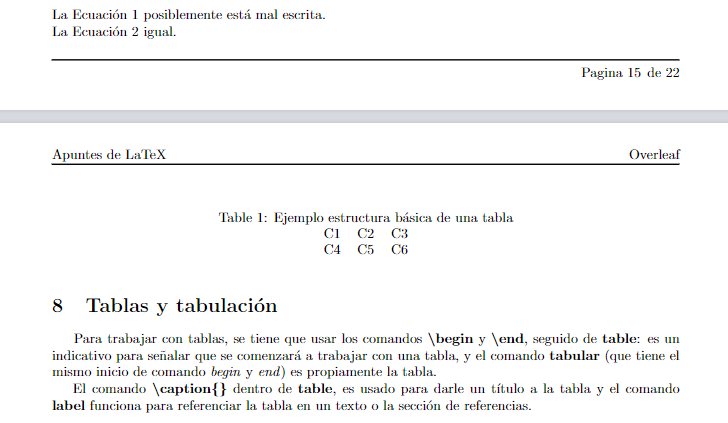
\includegraphics[width=\textwidth]{recursos/tablas_mal pos_1.png}
    \end{center}
\end{figure}
\begin{figure}[H]
    \begin{center}
        \caption{Mal posicionamiento de tablas, figuras u otros objetos 2}
        \label{fig: 3}
        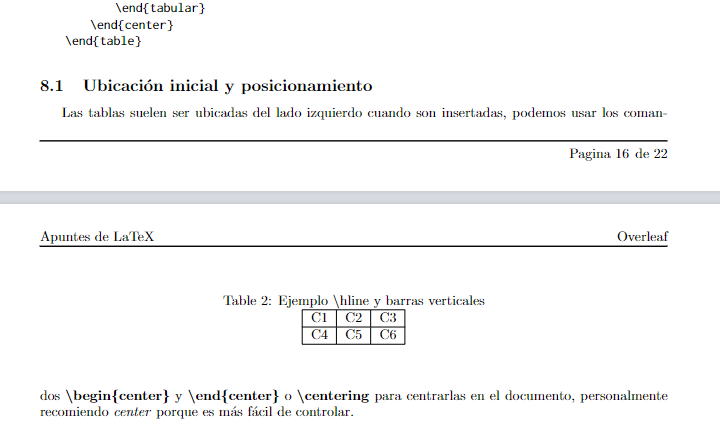
\includegraphics[width=\textwidth]{recursos/tablas_mal pos_2.png}
    \end{center}
\end{figure}

Las tablas que vemos en las imágenes anteriores son las que ya pusimos previamente, pero con un posicionamiento por defecto. Vemos que la Figura \ref{fig: 2} posiciona la tabla al principio de la página 15, previo a la sección de Tablas y tabulación; la Figura \ref{fig: 3} posiciona otra tabla al principio de la siguiente página, no donde nosotros lo deseamos.

Podemos pasar un parámetro de posicionamiento entre corchetes a \LaTeX dónde queremos la tabla, en todas las tablas usadas en este documento se utiliza el parámetro \textit{H}, esto debido a que permite que la tabla se ponga justo a continuación del último objeto o texto donde estuvimos posicionados, respetando el espacio de los objetos o textos a continuación. A continuación se muestra la lista de parámetros de posicionamiento:
\begin{enumerate}
    \item \textbf{h}: pone la tabla aproximadamente aquí.
    \item \textbf{p}: pone la tabla en una página especial, solo para tablas.
    \item \textbf{t}: pone la tabla en la parte superior de la página.
    \item \textbf{b}: pone la tabla en la parte inferior de la página
    \item \textbf{!}: fuerza el posicionamiento de la tabla en base a los parámetros listados aquí.
    \item \textbf{H}: pone la tabla exactamente aquí. Requiere del paquete \textbf{float} para poder ser utilizado.
\end{enumerate}
\begin{lstlisting}
    \begin{document}
        % Parámetro entre corchetes ([]) con el valor H para
        % posicionar estrictamente en dicha posición al
        % objeto.
        \begin{table}[H]
        
        \end{table}
    \end{document}
\end{lstlisting}

\textit{Nota}: personalmente recomiendo el parámetro H, posiciona la tabla donde queremos y respeta el espacio del resto del contenido del documento.

En ocasiones, cuando se está escribiendo un documento y se está trabajando con tablas, estas pueden chocar con el posicionamiento o espacio de las imágenes, por ejemplo, si tenemos una imagen, en seguida una tabla y luego una nueva sección o subsección, en vez de seguir ese orden, puede que ocurra que aparezca la imagen, la sección y luego la tabla, cosa que no va de acuerdo al orden que buscamos, para solucionar eso, puede insertar el comando \textbf{\textbackslash{newpage}} entre el fin de la imagen y el inicio de la tabla para lograr acomodar las cosas.

Otra solución es utilizar el parámetro entre corchetes ([]) con el valor H para las figuras, imágenes o ecuaciones:
\begin{lstlisting}
    \begin{document}
        Imagen
        \begin{figure}[H]
        
        \end{figure}
        Tabla
        \begin{table}[H]
        
        \end{table}
    \end{document}
\end{lstlisting}

De esta manera, ambos objetos respetan su propio posicionamiento y espacio, sin chocar ni afectar al resto de objetos o textos.
\begin{lstlisting}
    \begin{table}[H]
        \begin{center}
            \caption{Ejemplo de tabla con formato APA}
            \label{tab: 4}
            \begin{tabular}{l l l l}
                \hline
                Título 1 & Título 2 & Título 3 & Título4 \\
                \hline
                aaaaaaaaaaa         & bbbbbbbbbbbb  & cccccccc      & lorem impsum \\
                prueba 1            & prueba 2      & prueba tres   & prueba four \\
                texto de relleno    & rellenando    & info adicional& oh yeah \\
                \hline
            \end{tabular}
        \end{center}
    \end{table}
\end{lstlisting}
\begin{table}[H]
    \begin{center}
        \caption{Ejemplo de tabla con formato APA}
        \label{tab: 4}
        \begin{tabular}{l l l l}
            \hline
            Título 1 & Título 2 & Título 3 & Título4 \\
            \hline
            aaaaaaaaaaa         & bbbbbbbbbbbb  & cccccccc      & lorem impsum \\
            prueba 1            & prueba 2      & prueba tres   & prueba four \\
            texto de relleno    & rellenando    & info adicional& oh yeah \\
            \hline
        \end{tabular}
    \end{center}
\end{table}

La Tabla \ref{tab: 4} tiene un formato parecido a lo establecido al formato APA, esto es un ejemplo de como trabajar de forma sencilla con las tablas.


\subsection{Referenciar tablas en el texto}

Para poder referenciar en texto una tabla, es recomendable poner el texto de referencia dentro del comienzo de la tabla y previo del comienzo de \textbf{tabular}, antes de centrarla si es que se quiere centrar, para que, si se mueve la tabla, el texto de referencia se vaya con ella también, ya que si se pone afuera, el texto puede no quedar junto o cerca a la tabla.


\subsection{Ancho fijo de columnas}

Para que una tabla tenga columnas con un ancho fijo, se utiliza el paquete \textbf{array}.
\begin{center}
    \textit{\textbackslash{usepackage\{array\}}}
\end{center}

El tamaño del ancho de columna se indica dentro de llaves en las llaves donde se indica la alineación del contenido de las columnas, se tiene que tener conocimiento sobre las unidades de medida de \LaTeX.
\begin{center}
    \textbackslash{begin\{tabular\}\{m\{5cm\} m \{3cm\} m\{1cm\}\}}
\end{center}

En esta ocasión, como podemos recordar de los parámetros de las tablas convencionales (l, c, r), en este caso dejamos de lado los parámetros de alineación del contenido de columnas y los sustituiremos por los siguientes:
\begin{itemize}
    \item \textbf{m}: alinea el texto en medio de la columna.
    \item \textbf{b}: alinea el texto en la parte inferior de la columna.
    \item \textbf{p}: alinea el texto en la parte superior de la columna.
\end{itemize}
\begin{lstlisting}
    \begin{table}[H]
        \begin{center}
            \caption{Ejemplo de tabla con ancho de columna fijo}
            \label{tab: 5}
            \begin{tabular}{|m{5cm}|m{3cm}|m{1cm}|}
                \hline
                1   & 2 & 3 \\
                4   & 5 & 6 \\
                \hline
            \end{tabular}
        \end{center}
    \end{table}
\end{lstlisting}
\begin{table}[H]
    \begin{center}
        \caption{Ejemplo de tabla con ancho de columna fijo}
        \label{tab: 5}
        \begin{tabular}{|m{5cm}|m{3cm}|m{1cm}|}
            \hline
            1   & 2 & 3 \\
            4   & 5 & 6 \\
            \hline
        \end{tabular}
    \end{center}
\end{table}

La Tabla \ref{tab: 5} tiene ancho de de columna de 5cm, 3cm y 1cm (izquierda a derecha).


\subsection{Combinar filas y columnas}

Se requiere del paquete \textbf{multirow} para poder combinar columnas y filas.
\begin{center}
    \textit{\textbackslash{usepackage\{multirow\}}}
\end{center}

Se debe tener cuidado con los parámetros que reciben los comandos \textbf{\textbackslash{multirow\{\}\{\}\{\}}} y \\ \textbf{\textbackslash{multicolumn\{\}\{\}\{\}}} ya que varían un poco: para ambos, el primer parámetro recibe cuántas columnas o filas se van a combinar y el tercero indica el texto o contenido de dichas filas o columnas combinadas, el segundo parámetro varia dependiendo si se combina filas o columnas, para el primer caso, el parámetro recibe el ancho de fila (utilizando unidades de \LaTeX) y, para el segundo caso, recibe la alineación de las columnas (l, c, r):
\begin{lstlisting}
    \begin{table}[H]
        \begin{center}
            \caption{Ejemplo con tabla con columnas combinadas}
            \label{tab: 6}
            \begin{tabular}{c|c|c}
                \hline
                \multicolumn{3}{c}{3 celdas combinadas} \\
                \hline
                1   & 2 & 3 \\
                4   & 5 & 6 \\
                \hline
            \end{tabular}
        \end{center}
    \end{table}
    
    \begin{table}[H]
        \begin{center}
            \caption{Ejemplo con tabla con filas combinadas}
            \label{tab: 7}
            \begin{tabular}{m{5cm}|m{3cm}|m{1cm}}
                \hline
                1   & 2 & 3 \\
                \hline
                \multirow{2}{5cm}{2 filas combinadas}   & 4 & 5 \\
                &   6 & 7 \\
                \hline
                8   & 9 & 10 \\
                \hline
            \end{tabular}
        \end{center}
    \end{table}
\end{lstlisting}

\textit{Nota}: fijarse bien en como se distribuyen los elementos de cada celda si se desea combinar, ya sea filas o columnas, en el ejemplo anterior, por ejemplo, dependiendo si la tabla tendrá tres columnas, \textit{multicolumn} solo puede tomar como máximo tres columnas a combinar, si tiene cinco filas, \textit{multicolumn} se puede poner en cualquiera de esas cinco columnas.
\begin{table}[H]
    \begin{center}
        \caption{Ejemplo con tabla con filas combinadas}
        \label{tab: 6}
        \begin{tabular}{c|c|c}
            \hline
            \multicolumn{3}{c}{3 celdas combinadas} \\
            \hline
            1   & 2 & 3 \\
            4   & 5 & 6 \\
            \hline
        \end{tabular}
    \end{center}
\end{table}
\begin{table}[H]
    \begin{center}
        \caption{Ejemplo con tabla con columnas combinadas}
        \label{tab: 7}
        \begin{tabular}{m{5cm}|m{3cm}|m{1cm}}
            \hline
            1   & 2 & 3 \\
            \hline
            \multirow{2}{5cm}{2 filas combinadas}   & 4 & 5 \\
            &   6 & 7 \\
            \hline
            8   & 9 & 10 \\
            \hline
        \end{tabular}
    \end{center}
\end{table}

Repetimos, se debe tener cuidado combinando filas y columnas, para el primer caso, y con un ancho de columna fijo, el ancho de la columna donde se combinarán filas debe coincidir, tanto en la tabla, como en el comando \textbf{multirow} (\textit{Tabla \ref{tab: 6}}), y el número de columnas a combinar debe coincidir con el número real de columnas en una tabla con \textbf{multicolumn} (\textit{Tabla \ref{tab: 7}}).

\section{Figuras}

Las \textbf{figuras} son muy similares a las imágenes en \LaTeX, solo que este requiere de los comandos \textbf{\textbackslash{begin}} y \textbf{\textbackslash{end}}, seguido de \textbf{\{figure\}} para indicar una figura, los corchetes de ubicación [] también hacen aparición aquí, se requiere el paquete \textbf{graphicx}, importar las imágenes a esta plataforma para así adjuntarlas al documento.

Al igual que las imágenes, se adjuntan utilizando el comando \textbf{\textbackslash{includegraphics\{\}[]}}, que de igual forma, tiene el parámetro del tamaño entre corchetes y la figura propiamente dentro de llaves, la cual debe haber sido importada a esta plataforma previamente. La \textit{Figura \ref{fig: 4}} es el ejemplo de una imagen contenida por una figura:
\begin{lstlisting}
    \begin{figure}[H]
        \begin{center}
            \includegraphics [width=10cm]{ejemplo_latex.png}
        \end{center}
    \end{figure}
\end{lstlisting}
\begin{figure}[H]
    \begin{center}
        \caption{Figura de ejemplo}
        \label{fig: 4}
        \includegraphics[width=10cm]{recursos/ejemplo_latex.png}
    \end{center}
\end{figure}

\textit{Nota}: se recomienda trabajar las imágenes como figuras, ya que este contenedor permite asignarle nombres y etiquetas a las imágenes, como se ve en el ejemplo anterior.



\section{Comandos personalizados}

El comando \textbf{\textbackslash{newcommand}} nos permite tomar otros comandos y crear uno nuevo o uno personalizados, de tal forma que nos ahorre algo de tiempo, escritura y código.


\subsection{Sin parámetros}

Supongamos que queremos un acceso más rápido para el comando \textbf{\textbackslash{mathbb}} (previamente debimos haber agregado el paquete \textbf{amsfonts} para que este comando pudiera servir), para escribir el símbolo de los números reales, utilizamos \textit{newcommand\{\}\{\}}, en el primer par de llaves se escribe \textbf{\textbackslash}, seguido por el nombre que le darás a este nuevo comando, y en las segundas llaves, escribimos el comando que se ejecutará cuando llames al comando que apenas se está creando; no olvide que la creación de nuevos comandos puede ser antes o después al comienzo del documento:
\begin{lstlisting}
    \usepackage{asmfonts}
    
    \newcommand{\R}{\mathbb{R}}
    
    \begin{document}
        \R
    \end{document}
\end{lstlisting}

\newcommand{\R}{\mathbb{R}}

El resultado de usar nuestro nuevo comando creado \textbf{\textbackslash{R}} es: los números reales son $\R$


\subsection{Con parámetros}

Podemos crear comandos nuevos que involucren la entrada de datos para que estos desplieguen algún texto o resultado. En este caso buscamos crear un comando que reciba dos números o letras para formar un vector, involucraremos la creación de una matriz durante el camino, para ello, utilizamos el comando \textbf{newcommand\{\}[]\{\}}, el primero y último es lo mismo que el anterior ejemplo, el segundo parámetro se encuentra entre corchetes, y en este se definirán el número de parámetros para el nuevo comando (si son tres parámetros, para pasárselos al comando que se ejecutará cuando llamemos al que estamos creando actualmente, debemos poner el símbolo \#, seguido del número de parámetro que deseemos: \#1, \#2, \#3, ..., \#n):
\begin{lstlisting}
    \begin{document}
        \newcommand{\M}[2]{
            \begin{bmatrix}
	            #1\\
	            #2\\
            \end{bmatrix}
        }
    \end{document}
\end{lstlisting}
\newcommand{\M}[2]{\begin{bmatrix}
	#1\\
	#2\\
\end{bmatrix}
}

Primer intento, le pasamos a \textbf{\textbackslash{M\{\}\{\}}} los valores 1 y 2, el resultado es: $\M{1}{2}$

Segundo intento, le pasamos a \textbf{\textbackslash{M\{\}\{\}}} los valores a y b, el resultado es: $\M{a}{b}$

\section{Matemáticas}

Las matemáticas, fórmulas y ecuaciones son el área fuerte de \LaTeX.


\subsection{Fórmulas y área de trabajo de fórmulas}
\begin{itemize}
    \item \textbf{Sin espacio dedicado}: una ecuación o fórmula, puesta en el documento de forma sencilla y sin dedicarle un espacio dedicado, requiere de dos símbolos de dolar (\textbf{\$}): \$ecuación\$. Las siguientes dos ecuaciones solamente están puestas con un \$ al inicio y al final, una tras otra, sin comando de salto de línea:
    \begin{center}
        \textit{
            \$e\textasciicircum{2}\$, \$e\textasciicircum{\{1/2\}}\$ \\
            $e^2$, $e^{1/2}$
        }
    \end{center}
    \item \textbf{Con espacio dedicado}: dos símbolos de dolar (\textbf{\$\$}) al inicio y final indica el comienzo de un área de trabajo para ecuaciones, la siguiente ecuación están dentro de dicho área y por ello están centradas en el documento:
    \begin{center}
        \$\$e\textasciicircum\{1/3\textbackslash{pi}\}\$\$
    \end{center}
    $$e^{1/3\pi}$$
    \item \textbf{El entorno Equation}: los comandos \textbf{\textbackslash{begin\{\}}} y \textbf{\textbackslash{end\{\}}}, donde entre sus llaves se escribe \textbf{equation}, funcionan para así tener ecuaciones centradas y enumeradas.
    \begin{center}
        \textit{
            \textbackslash{begin\{equation\}} \\
            \textbackslash{Pi}=3.1416 \\
            \textbackslash{end\{equation\}}}
    \end{center}
    \begin{equation}
        \label{ec: 3}
        \Pi=3.1416
    \end{equation}
    \item El comando \textbf{cdot} pone un punto, en este caso multiplicación, dentro de un texto, fórmula o ecuación.
    \begin{center}
        \$\$\textbackslash{cdot}\$\$\\
        4\textbackslash{cdot}5
    \end{center}
    $$4\cdot5$$
    \item Al principio del documento, podemos usar paquetes dentro del documento para hacerlo más rico y completo, uno de ellos es \textbf{amsmath}, te proporciona más comandos matemáticos\begin{center}\textit{\textbackslash{usepackage\{amsmath\}}}\end{center}
\end{itemize}


\subsection{Alineación de ecuaciones: Align, Slip y Multiline}


\subsubsection{Align}

Si buscamos que nuestras ecuaciones se mantengan alineadas correctamente, centradas y enumeradas, podemos utilizar los comandos \textbf{\textbackslash{begin\{\}}} y \textbf{\textbackslash{end\{\}}}, donde entre sus llaves se escribe \textbf{align}. Esto puede ser usado como cuando se muestra el desarrollo de una ecuación, integral, derivada u otro problema matemático, por ejemplo, el desarrollo de un límite:
\begin{lstlisting}
    \begin{align}
        \label{ec: ecuacion3}
        e=\lim_{n\to\infty}\left(1+\frac{1}{n}\right)^n \\
        \label{ec: ecuacion4}
        =\lim_{n\to 0}(1+t)^\frac{1}{t}
    \end{align}
\end{lstlisting}
\begin{align}
    \label{ec: 4}
    e=\lim_{n\to\infty}\left(1+\frac{1}{n}\right)^n\\
    \label{ec: 5}
    =\lim_{n\to 0}(1+t)^\frac{1}{t}
\end{align}

La \textit{Ecuación \ref{ec: 4}} y \textit{\ref{ec: 5}} muestran un ejemplo de como podríamos tener presente un ejemplo de un desarrollo de ecuaciones sin alinear (símbolos de igualdad disparejos) y que, además, al ser un desarrollo de un solo problema, se muestran como ecuaciones independientes. Podemos lograr que este desarrollo se muestre como una sola ecuación.


\subsubsection{Slipt}

Para hacer que las ecuaciones dentro del desarrollo de una misma estén correctamente alineadas con respecto al símbolo de igualdad, se pone el símbolo \& antes de todos los símbolos de igualdad de todo el desarrollo para que así, las siguientes ecuaciones se alineen correctamente y, en vez de usar \textit{align} dentro de \textit{begin} y \textit{end}, volvemos a usar \textit{equation}, además de que toda la ecuación estará dentro de otro comando begin y end donde su contenido ahora será \textbf{slipt}.
\begin{lstlisting}
    \begin{equation}
        \label{ec: 6}
        \begin{split}
            e&=\lim_{n\to\infty}\left(1+\frac{1}{n}\right)^n \\
            &=\lim_{n\to 0}(1+t)^\frac{1}{t}
        \end{split}
    \end{equation}
\end{lstlisting}
\begin{equation}
    \label{ec: 6}
    \begin{split}
        e&=\lim_{n\to\infty}\left(1+\frac{1}{n}\right)^n \\
        &=\lim_{n\to 0}(1+t)^\frac{1}{t}
    \end{split}
\end{equation}

La \textit{Ecuación \ref{ec: 6}} ahora si está bien centrada y enumerada a un solo desarrollo de problema matemático.


\subsubsection{Multiline}

En caso de tener una ecuación muy larga, se puede usar los comandos \textbf{\textbackslash{begin\{\}}} y \textbf{\textbackslash{end\{\}}}, donde entre sus llaves se escribe \textbf{multiline} para hacer saltos de línea a lo largo de toda la ecuación, para lograr esto, supongamos que tenemos una ecuación matemática larga y la queremos dividir en cuatro partes y ponerlas una debajo de otra, para separar estas partes las encerramos entre \textbackslash\textbackslash (al inicio y final) y con eso basta, todas las partes deben ser encerradas entre estas barras, tanto la primera (inicial) como la última (final).

La estructura es exactamente la misma al ejemplo anterior, lo único que cambia es precisamente el tipo de \textit{begin} y \textit{end} (con la palabra que ya mencionamos anteriormente) y se usan dos diagonales invertidas en los puntos de la ecuación donde se quiera hacer una separación.
\begin{lstlisting}
    \begin{multline}
        \label{ec: ecuacion6}
        \frac{1}{2}+\frac{2}{2}+\frac{2}{2}+\frac{3}{2}+\frac{4}{2}+\frac{5}{2}+\frac{6}{2}+\frac{7}{2}+\frac{8}{2}+\frac{9}{2}+\frac{10}{2}+\frac{1}{3}+\frac{2}{3}+\frac{3}{3}+\frac{4}{3}+\frac{5}{3}+\frac{6}{3}+\frac{7}{3}+\frac{9}{3}+\frac{10}{3}=0
    \end{multline}
\end{lstlisting}
\begin{multline}
        \label{ec: 7}
        \frac{1}{2}+\frac{2}{2}+\frac{2}{2}+\frac{3}{2}+\frac{4}{2}+\frac{5}{2}+\frac{6}{2}+\frac{7}{2}+\frac{8}{2}+\frac{9}{2}+\frac{10}{2}+\frac{1}{3}+\frac{2}{3}+\frac{3}{3}+\frac{4}{3}+\frac{5}{3}+\frac{6}{3}+\frac{7}{3}+\frac{9}{3}+\frac{10}{3}=0
\end{multline}

La \textit{Ecuación \ref{ec: 7}} es muy larga y no tiene espaciado dentro de \textbf{multiline}.
\begin{lstlisting}
    \begin{multline}
        \label{ec: ecuacion7}
        \\\frac{1}{2}+\frac{2}{2}+\frac{2}{2}+\frac{3}{2}+\frac{4}{2}\\+\frac{5}{2}+\frac{6}{2}+\frac{7}{2}+\frac{8}{2}+\frac{9}{2}\\+\frac{10}{2}+\frac{1}{3}+\frac{2}{3}+\frac{3}{3}+\frac{4}{3}\\+\frac{5}{3}+\frac{6}{3}+\frac{7}{3}+\frac{9}{3}+\frac{10}{3}=0\\
    \end{multline}
\end{lstlisting}
\begin{multline}
    \label{ec: 8}
    \\
    \frac{1}{2}+\frac{2}{2}+\frac{2}{2}+\frac{3}{2}+\frac{4}{2} \\
    +\frac{5}{2}+\frac{6}{2}+\frac{7}{2}+\frac{8}{2}+\frac{9}{2} \\
    +\frac{10}{2}+\frac{1}{3}+\frac{2}{3}+\frac{3}{3}+\frac{4}{3} \\
    +\frac{5}{3}+\frac{6}{3}+\frac{7}{3}+\frac{9}{3}+\frac{10}{3}=0 \\
\end{multline}

La \textit{Ecuación \ref{ec: 8}} está dividida en cuatro partes, centrada y con numeración de ecuación, todo gracias a \textbf{multiline}.


\subsection{Fracciones}


\subsubsection{Sencillas}
\begin{itemize}
    \item Se utiliza el comando de \textbf{\textbackslash{frac\{\}\{\}}} para una fracción, es otra forma de escribirlas: el primer par de llaves es el numerador, el segundo par el denominador.
    \begin{center}
        \textit{\$\$(\textbackslash{frac\{1+\}\{\textbackslash{frac\{3\}\{n\}}\}})\$\$}
    \end{center}
    $$\frac{2}{5}$$
    $$(1+\frac{3}{n})$$
    \item La ecuación anterior presenta los paréntesis muy pequeños, se aumentan con el comando \textbf{\textbackslash{left}} y \textbf{\textbackslash{right}}, ambos al principio y final de su respectivo paréntesis. En otras palabras, paréntesis que se ajustan automáticamente.
    \begin{center}
        \textit{\$\$\textbackslash{left}(\textbackslash{frac\{1+\}\{\textbackslash{frac\{3\}\{n\}}\}}\textbackslash{right})\$\$}
    \end{center}
    $$\left(1+\frac{1}{3}\right)^n$$
\end{itemize}


\subsubsection{Fracciones en fracciones}
\begin{itemize}
    \item No es algo más que poner dentro de las llaves de \textit{frac} otro comando \textbf{frac}, así como se desee para poner fracciones dentro de fracciones.
    \begin{center}
        \textit{\$\$\textbackslash{frac\{1\}\{\textbackslash{frac\{1+\}\{\textbackslash{frac\{2\}\{2n+1\}}\}}\}}\$\$}
    \end{center}
    $$\frac{\frac{1}{3}}{\frac{2}{5}}$$
    $$\frac{1}{1+\frac{2}{2n+1}}$$
    \item Si se pone el comando \textbf{ddots} crea tres puntos diagonales que significan que una ecuación continua un camino con patrón visible:
    $$\ddots$$
\end{itemize}


\subsection{Límites}

Los límites se escriben utilizando el comando \textbf{\textbackslash{lim}}. Para agregar valores debajo de la palabra \textit{lim}, escribimos el comando \textit{\textbackslash{lim}}, seguido usamos el guión bajo (\_), entre llaves, escribimos la expresión del límite (separados por el comando \textbf{\textbackslash{to}}). El primero ejemplo a continuación es  un límite simple sin valores, el segundo ya tiene un valor escrito debajo de la palabra lim (n a infinito y n a 8):
\begin{center}
    \textit{
        \$\$\textbackslash{lim}\textbackslash{left}(1+\textbackslash{frac\{1\}\{3\}}\textbackslash{right})\textasciicircum n\$\$ \\
        \$\$\textbackslash{lim}\_\{n\textbackslash{to}\textbackslash{infty}\}\textbackslash{left}(1+\textbackslash{frac\{1\}\{3\}}\textbackslash{right})\textasciicircum n\$\$ \\
        \$\$\textbackslash{lim}\_\{n\textbackslash{to}8\}\textbackslash{left}(1+\textbackslash{frac\{1\}\{3\}}\textbackslash{right})\textasciicircum n\$\$
    }
\end{center}
$$\lim \left(1+\frac{1}{3}\right)^n$$
$$\lim_{n\to\infty} \left(1+\frac{1}{3}\right)^n$$
$$\lim_{n\to8} \left(1+\frac{1}{3}\right)^n$$

\textit{Nota}: el comando \textbf{\textbackslash{infty}} es un símbolo de infinito en el ambiente de matemáticas.


\subsection{Raíces}

Para poner una raíz se usa el comando \textbf{\textbackslash{sqrt[]\{\}}}. Este comando tiene dos parámetros, uno dentro de corchetes y otro dentro de llaves, el primero es para indicar el nivel de raíz (raíz cuadrada/cúbica/cuarta...\\), y el otro para el contenido (raíz de 4, 16, 25, x...), pero si se quiere una raíz simple podemos usar solo los parámetros entre llaves. El símbolo de factorial no tiene un comando como tal, solo es el símbolo !.
\begin{center}
    \textit{
        \$\$\textbackslash{sqrt\{25\}}\$\$ \\
        \$\$\textbackslash{sqrt[3]\{4!\}}\$\$
    }
\end{center}
$$\sqrt{25}$$
$$\sqrt[3]{4}$$
$$\sqrt[3]{4!}$$


\subsection{Sumatorias}

Las sumatorias requieren el comando \textbf{\textbackslash{sum}}, para poner valores debajo de la sumatoria se aplica lo mismo que con los límites, que es poner guión bajo seguido de llaves(\_\{\}), para poner valores encima de la sumatoria, debemos poner el símbolo de elevar a tal potencia y, entre llaves, el valor correspondiente (\textasciicircum{\textbackslash{infty}}, 10, 100,...).
\begin{center}
    \textit{\$\$\textbackslash{sum\_\{n=0\}}\textasciicircum{\{\textbackslash{infty}\}} \textbackslash{frac\{1\}\{n!\}}\$\$}
\end{center}
$$\sum_{n=0}^{\infty} \frac{1}{n!}$$


\subsection{Integrales}

Se usa el comando \textbf{\textbackslash{int}} para integrales, si es definida, se usa el guión bajo y potencia para indicar los valores definidos de la integral, si se quiere más de una integral en la misma, se ponen todas las i's que se quieran al inicio del comando (\textit{iiint}).
\begin{itemize}
    \item Definidas
    \begin{center}
        \textit{\$\$\textbackslash{int\_1\textasciicircum{1}}f(x)dx\$\$}
    \end{center}
    $$\int_1^2f(x)dx$$
    \item Indefinidas
    \begin{center}
        \textit{\$\$\textbackslash{int f(x)dx}\$\$}
    \end{center}
    $$\int f(x)dx$$
    \item Múltiples integrales
    \begin{center}
        \textit{\$\$\textbackslash{iiint\_0\textasciicircum{2}}f(x,y,z)dxdydz\$\$}
    \end{center}
    $$\iiint_0^2f(x,y,z)dxdydz$$
\end{itemize}


\subsection{Vectores}

Se usa el comando \textbf{\textbackslash{vec\{\}}}, dentro de sus llaves ponemos el nombre del vector, o la letra que lo caracterizará, si el vector tiene valores, estos valores se indican usando el nombre del vector, seguido de un guión bajo y el número del valor.
\begin{itemize}
    \item Símbolo
    \begin{center}
        \textit{\$\$\textbackslash{vec\{a\}}\$\$}
    \end{center}
    $$\vec{a}$$
    \item Con valores
    \begin{center}
        \textit{\$\$\textbackslash{vec\{a\}}=\textless v\_1, v\_2, v\_3\textgreater\$\$}
    \end{center}
    $$\vec{v}=<v_1, v_2, v_3>$$
    \item Con operaciones
    \begin{center}
        \textit{\$\$\textbackslash{vec\{a\}}\textbackslash{cdot}\textbackslash{vec\{b\}}\$\$}
    \end{center}
    $$\vec{a}\cdot\vec{b}$$
\end{itemize}


\subsection{Matrices}

Se usa el comando \textbf{\textbackslash{begin\{\}}} y \textbf{\textbackslash{end\{\}}}, y dentro de sus llaves se usa el comando \textbf{bmatrix} para crearla, cada item dentro de una fila se separa con el símbolo \textbf{\&}, si la matriz tiene tres elementos en la primera fila, se separan con dicho carácter, y para finalizar dicha fila, se ponen las dos diagonales invertidas \textbackslash\textbackslash (salto de línea), así sucesivamente hasta armar la matriz deseada.
\begin{lstlisting}
    $$\begin{bmatrix}
        1 & 2  & 3  & 4 \\
        5 & 6  & 7  & 8 \\
        9 & 10 & 11 & 0 \\
    \end{bmatrix}$$
\end{lstlisting}
$$\begin{bmatrix}
    1&2&3&4\\
    5&6&7&8\\
    9&10&11&0\\
\end{bmatrix}$$


% Agrega referencias al documento.
\newpage\printbibliography[heading=bibintoc, title={Referencias}]

% Final del documento.
\end{document}